\begin{enumerate}[label=\thesection.\arabic*.,ref=\thesection.\theenumi]
\numberwithin{equation}{enumi}
\item Show by plotting the output that a lead compensator reduces settling time of a control system.\\
\solution considering the above discussed control system \eqref{eq:ee18btech11021_gs} and the lead compensator.

Unity feedback system - 
\begin{figure}[h]
\begin{center}
\resizebox{\columnwidth}{!}{\tikzstyle{block} = [draw, fill=blue!20, rectangle, 
    minimum height=0.7cm, minimum width=0.7cm]
\tikzstyle{sum} = [draw, fill=blue!20, circle, node distance=1cm]
\tikzstyle{input} = [coordinate]
\tikzstyle{output} = [coordinate]
\tikzstyle{pinstyle} = [pin edge={to-,thin,black}]

\begin{tikzpicture}[auto, node distance=2.5cm,>=latex']
    % We start by placing the blocks
    \node [input, name=input] {};
    \node [sum, right of=input] (sum) {};
    \node [block, right of=sum] (controller) {H(s)};
    \node [output, right of=controller] (output) {};


    \draw [draw,->] (input) -- node {$R(s)\ +$} (sum);
    \draw [->] (sum) -- node {$E(s)$} (controller);
    \draw [->] (controller) -- node [name=y] {$Y(s)$}(output);
  \draw [->] (y) -- ++ (0,-2) -| node [pos=0.99] {$-$} (sum);
 
\end{tikzpicture}}
\end{center}
\end{figure}

Compensated system - 
\begin{figure}[h]
\begin{center}
\resizebox{\columnwidth}{!}{

\tikzstyle{block} = [draw, fill=blue!20, rectangle, 
    minimum height=3em, minimum width=6em]
\tikzstyle{sum} = [draw, fill=blue!20, circle, node distance=1cm]
\tikzstyle{input} = [coordinate]
\tikzstyle{output} = [coordinate]
\tikzstyle{pinstyle} = [pin edge={to-,thin,black}]

% The block diagram code is probably more verbose than necessary
\begin{tikzpicture}[auto, node distance=2cm,>=latex']
    % We start by placing the blocks
    \node [input, name=input] {};
    \node [sum, right of=input] (sum) {};
    \node [block, right of=sum] (controller) {G(s)};
    \node [block, right of=controller,
           node distance = 4cm ] (system) {D(s)};
    % We draw an edge between the controller and system block to 
    % calculate the coordinate u. We need it to place the measurement block. 
    \draw [->] (controller) -- node[name=u] {$U(s)$} (system);
    \node [output, right of=system] (output) {};
    \coordinate [below of=u] (tmp);

    % Once the nodes are placed, connecting them is easy. 
    \draw [draw,->] (input) -- node {$R(s)\ +$} (sum);
    \draw [->] (sum) -- node {} (controller);
    \draw [->] (system) -- node [name=y] {$Y(s)$}(output);
    \draw [->] (y) |- (tmp) -| node[pos=0.99] {$-$} 
        node [near end] {} (sum);
\end{tikzpicture}

}
\end{center}
\end{figure}

Settling time - \\
It is the time required for the response to reach the steady state and stay within the specified tolerance bands around the final value. In general, the tolerance bands are 2\% and 5\%.

let,
\begin{align}
system-G(s) = \frac{1}{s(3s+1)}\\
lead\ compensator-D(s) = \frac{3(s+\frac{1}{3})}{(s+1)}
\end{align}
\begin{equation}
    \begin{split}
        hence, new\ system-G_{1}(s) = G(s)D(s)\\
        = \frac{1}{s(s+1)}
    \end{split}
\end{equation}

1). Unit impulse response - \\
a). without lead compensator - 
\begin{align}
G(s) = \frac{1}{(s)(3s+1)}\\
Y(s) = \frac{G(s)}{1+G(s).1}.R(s)\\
Y(s) = \frac{G(s)}{1+G(s).1}.1\\
Y(s) = \frac{1}{3s^2+s+1}\\
Y(s) = \frac{1}{3}\frac{1}{(s+\frac{1}{6})^2 + \frac{11}{36}}
\end{align}
taking inverse laplace transform, 
\begin{align}
y(t) = [\frac{2}{\sqrt{11}}e^{\frac{-t}{6}}sin(\frac{\sqrt{11}t}{6}))]u(t)
\end{align}

b). with lead compensator - 
\begin{align}
G(s) = \frac{1}{(s)(3s+1)}\\
D(s) = \frac{3(s+\frac{1}{3})}{(s+1)} \\
G_{1}(s) = \frac{1}{s(s+1)}\\
Y_{1}(s) = \frac{G_{1}(s)}{1+G_{1}(s)}.R(s)\\
Y_{1}(s) = \frac{G_{1}(s)}{1+G_{1}(s)}.1\\
Y_{1}(s) = \frac{1}{s^2+s+1}\\
Y_{1}(s) = \frac{1}{(s+\frac{1}{2})^2 + \frac{3}{4}} 
\end{align}
taking inverse laplace transform, 
\begin{align}
y(t) = [\frac{2}{\sqrt{3}}e^{\frac{-t}{2}}sin(\frac{\sqrt{3}t)}{2})]u(t)
\end{align}

2). unit step response - \\
a). without lead compensator - 
\begin{align}
G(s) = \frac{1}{(s)(3s+1)}\\
Y(s) = \frac{G(s)}{1+G(s).1}.R(s)\\
Y(s) = \frac{G(s)}{1+G(s)}.\frac{1}{s}\\
Y(S) = \frac{1}{(s)(3s^2+s+1)}\\
Y(s) = \frac{-3s-1}{3s^2+s+1} + \frac{1}{s}
\end{align}
\begin{equation}
\begin{split}
Y(s) = \frac{1}{s} - \frac{s+\frac{1}{6}}{(s+\frac{1}{6})^2 + \frac{11}{36}}\\ -\frac{1}{6}\frac{1}{(s+\frac{1}{6})^2  \frac{11}{36}}+
\end{split}
\end{equation}
taking inverse laplace transform, 
\begin{equation}
    \begin{split}
        y(t) = [1 - e^{\frac{-t}{6}}cos(\frac{\sqrt{11}t}{6})\\- \frac{1}{\sqrt{11}}e^{\frac{-t}{6}}sin(\frac{\sqrt{11}t}{6}) ]u(t)
    \end{split}
\end{equation}

b). with lead compensator - 
\begin{align}
G(s) = \frac{1}{(s)(3s+1)}\\
D(s) = \frac{3(s+\frac{1}{3})}{s+1} \\
G_{1}(s) = \frac{1}{s(s+1)}\\
Y_{1}(s) =\frac{G_{1}(s)}{1+G_{1}(s)}.R(s)\\
Y_{1}(s) =\frac{G_{1}(s)}{1+G_{1}(s)}.\frac{1}{s}\\
Y_{1}(s) = \frac{1}{s(s^2+s+1)}\\
Y_{1}(s) = \frac{-s-1}{s^2+s+1} + \frac{1}{s}
\end{align}
\begin{equation}
    \begin{split}
        Y_{1}(s) =  \frac{1}{s} - \frac{s+\frac{1}{2}}{(s+\frac{1}{2})^2+\frac{3}{4}}\\ - \frac{1}{2}\frac{1}{(s+\frac{1}{2})^2+\frac{3}{4}} + 
    \end{split}
\end{equation}

taking inverse laplace transform, 
\begin{equation}
    \begin{split}
        y(t) = [1 - e^{\frac{-t}{2}}cos(\frac{\sqrt{3}t}{2})\\- \frac{1}{\sqrt{3}}e^{\frac{-t}{2}}sin(\frac{\sqrt{3}t}{2}) ]u(t)
    \end{split}
\end{equation}


\begin{figure}
%\begin{subfigure}{\textwidth}
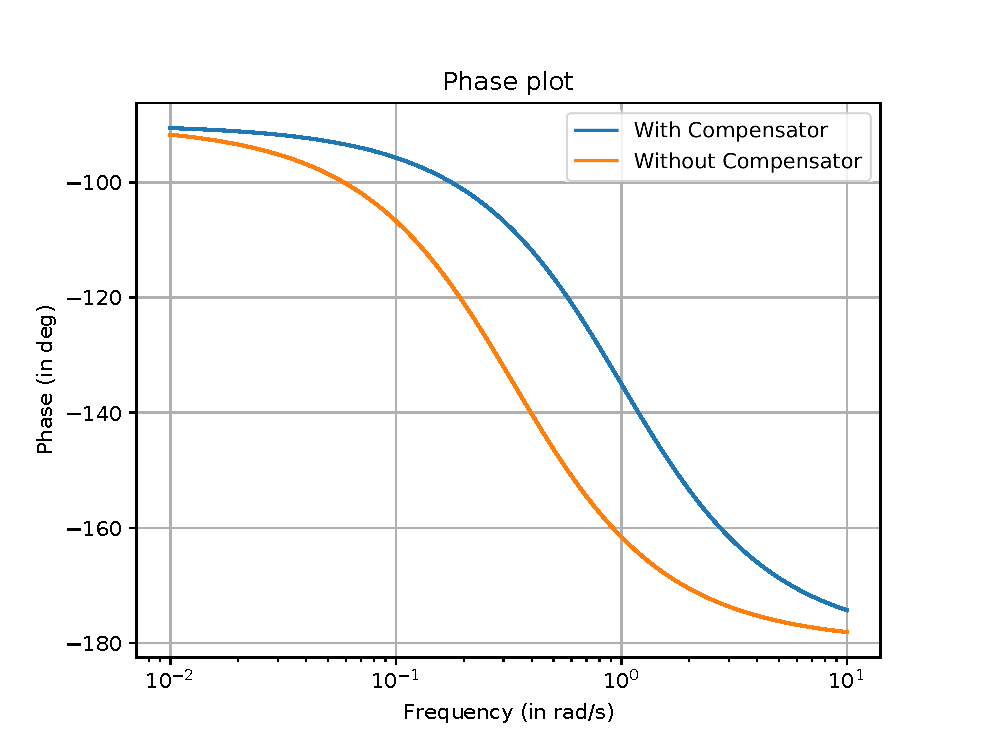
\includegraphics[width=1\linewidth, height=7cm ,inner]{./figs/ee18btech11027/lead_compensator_phase.eps} 
\label{fig:subim1}
%\end{subfigure}
\end{figure}


\begin{figure}
%\begin{subfigure}{\textwidth}
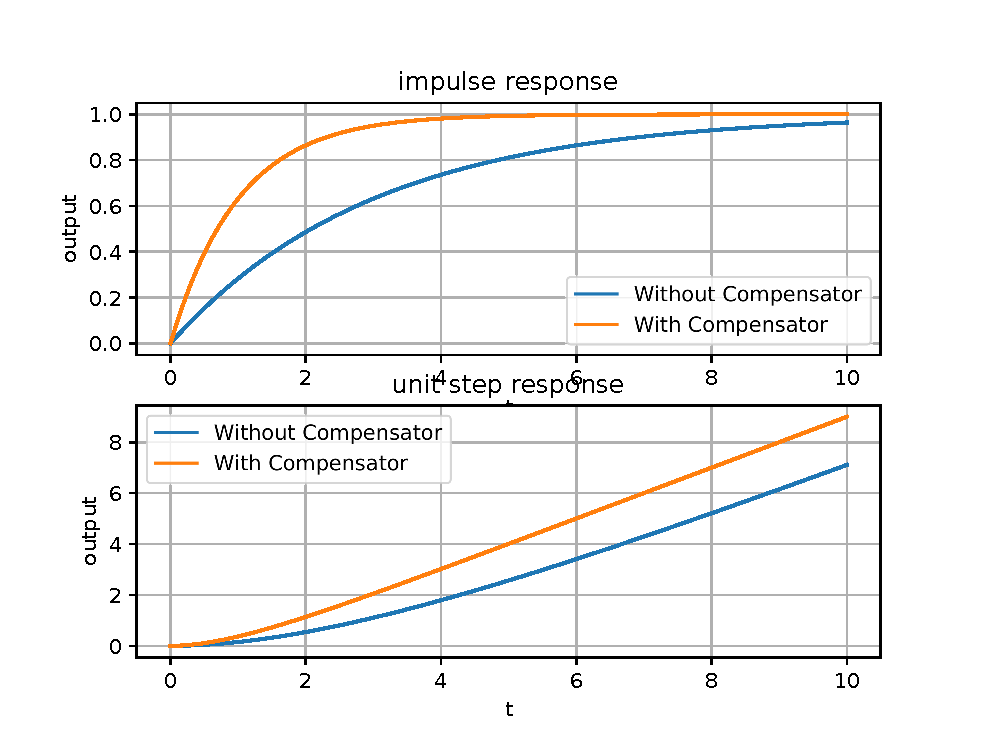
\includegraphics[width=1\linewidth, height=7cm ,inner]{./figs/ee18btech11027/settling_time.eps} 
\label{fig:subim1}
%\end{subfigure}
\end{figure}
Hence, from both examples we can see that settling time is reduced by using a lead compensator.

\item Theoritically state how the lead compensator reduces settling time.\\
\solution
Since lead compensator adds +ve phase for any value of frequency, the phase bode plot of compensated system is above the one which is without lead compensator.
\begin{align}
    \phi_m = 180 + \phi_{gain = 0}
\end{align}

as lead compensator adds additional phase
at all frequencies, 
$\phi_{gain = 0}$  gets increased, and hence\ phase\ margin.

Relation between phase margin and damping ratio.
\zeta = 0.01 $\times$ \phi_m

From this we get that damping factor also increases with phase margin.
\begin{align}
\implies damping\ is\ increased \\
\implies settling\ time\ decreased
\end{align}

\item Derive a relation between phase margin and damping ratio.\\
\solution
Consider a second order system,
\begin{align}
G(s) = \frac{\omega_n^2}{s^2+2\zeta\omega_ns+\omega_n^2} 
\end{align}

using value of $\phi_m$ to solve for $\zeta$.
set 20 $\log{|G(s)|}$ = -3dB to solve for \omega_n

using this equations we get,

\begin{align}
\phi_m = \tan^{-1}{\frac{2\zeta}{\sqrt{\sqrt{1+4\zeta^4} - 2\zeta^2}}}
\end{align}
a handy relation is - \zeta = 0.01\phi_m

\begin{figure}[h]
 \textbf{phase margin vs damping ratio}
\begin{subfigure}{\textwidth}
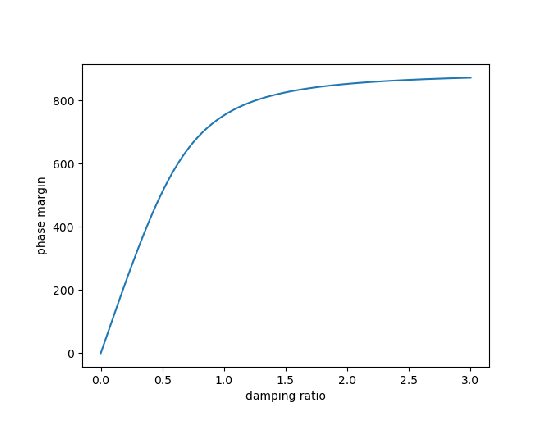
\includegraphics[width=1\linewidth, height=7cm ,inner]{./figs/ee18btech11027/realtion.eps} 
\label{fig:subim1}
\end{subfigure}
\end{figure}

Hence,for a lead compensator phase margin increases, therfore damping increases, resulting in reduced settling time.
Similarly if we use a lag compensator the settling time increases beacuse the phase margin decreases.

\end{enumerate}